%!TEX TS-program = xelatex
%!TEX encoding = UTF-8 Unicode

\documentclass[11pt,tikz,border=1]{standalone}
\usetikzlibrary{positioning}

\begin{document}
  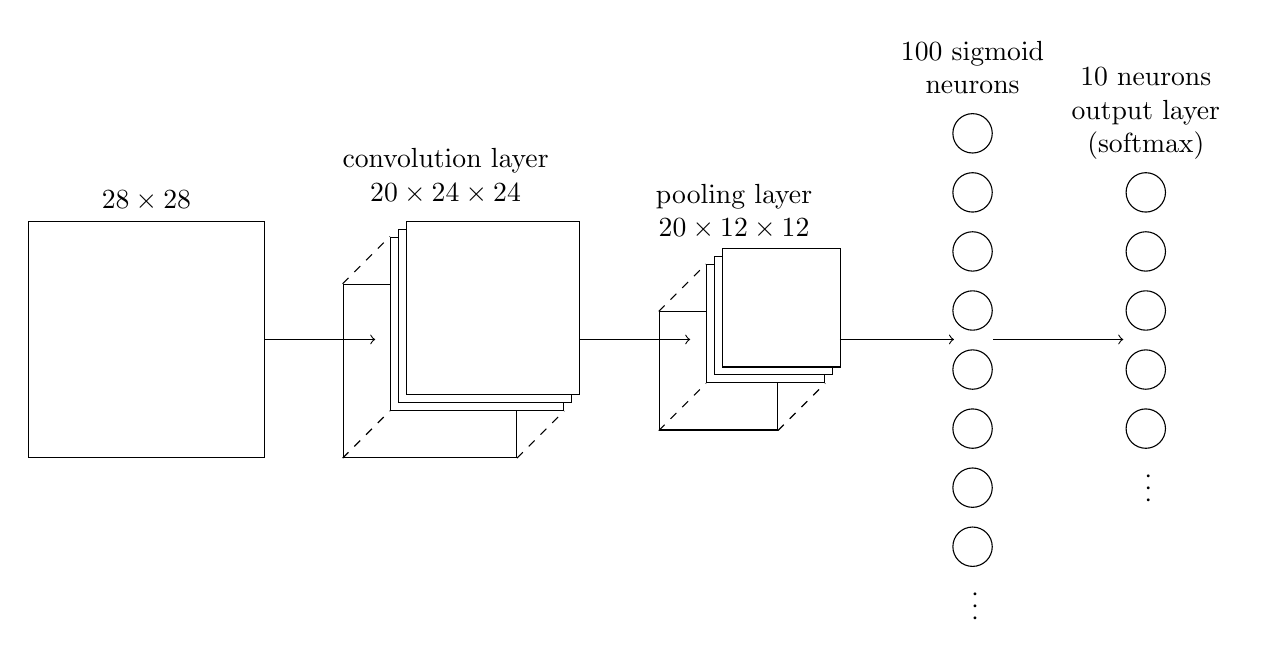
\begin{tikzpicture}[
    inputlayer/.style={rectangle,draw,fill=white,inner sep=0pt,minimum size=30mm},
    hiddenlayer/.style={rectangle,draw,fill=white,inner sep=0pt,minimum size=22mm},
    poolinglayer/.style={rectangle,draw,fill=white,inner sep=0pt,minimum size=15mm},
    neuron/.style={circle,draw,inner sep=0pt,minimum size=5mm}
    ]

    \node (input) [inputlayer,anchor=south west] at (0,0) {};

    \node (hidden0) [hiddenlayer,anchor=south west] at (4,0) {};
    
    \node (hidden1) [hiddenlayer,anchor=south west,xshift=6mm,yshift=6mm] at (hidden0.south west) {};
    \node (hidden2) [hiddenlayer,anchor=south west,xshift=1mm,yshift=1mm] at (hidden1.south west) {};
    \node (hidden3) [hiddenlayer,anchor=south west,xshift=1mm,yshift=1mm] at (hidden2.south west) {};
    
    \draw[dashed] (hidden0.north west) -- (hidden1.north west);
    \draw[dashed] (hidden0.south west) -- (hidden1.south west);
    \draw[dashed] (hidden0.south east) -- (hidden1.south east);
    
    \foreach \x in {0,1,2,3}
      \node (pooling\x) [poolinglayer,anchor=west,right=1.8 of hidden\x] {};

    \draw[dashed] (pooling0.north west) -- (pooling1.north west);
    \draw[dashed] (pooling0.south west) -- (pooling1.south west);
    \draw[dashed] (pooling0.south east) -- (pooling1.south east);

    \foreach \x in {0,...,7}
      \node(s\x) [neuron] at (12, 0.75 * \x - 1.125) {};

    \foreach \x in {0,...,4}
      \node(o\x) [neuron] at (14.2, 0.75 * \x + 0.375) {};

    \node [above] at (input.north) {$28 \times 28$};
    \node [above,xshift=-6mm] at (hidden3.north) {
      \begin{tabular}{c}
        convolution layer\\
        $20 \times 24 \times 24$
      \end{tabular}
    };
    \node [above,xshift=-5mm] at (pooling2.north) {
      \begin{tabular}{c}
        pooling layer\\
        $20 \times 12 \times 12$
      \end{tabular}
    };
    \node [above] at (s7.north) {
      \begin{tabular}{c}
        100 sigmoid\\
        neurons
      \end{tabular}
    };
    \node [above] at (o4.north) {
      \begin{tabular}{c}
        10 neurons\\
        output layer\\
        (softmax)
      \end{tabular}
    };
    \node [below,rotate=-90,xshift=5mm,yshift=1.75mm] at (s0.south) {$\ldots$};
    \node [below,rotate=-90,xshift=5mm,yshift=1.75mm] at (o0.south) {$\ldots$};
    
    \coordinate(a0) at (input.east);

    \draw[->] (a0) -- ++(1.4,0);
    \draw[->] (a0)++(4,0) -- ++(1.4,0);
    \draw[->] (a0)++(7.3,0) -- ++(1.45,0);
    \draw[->] (a0)++(9.25,0) -- ++(1.65,0);

  \end{tikzpicture} 
\end{document}
